\documentclass[11pt]{article}

% PACKAGES
\usepackage{microtype} % microtypography
%\usepackage{booktabs}  % tables
\usepackage{hyperref}  % urls
\usepackage{amsmath}
\usepackage{amsthm}
\usepackage{graphicx}
\usepackage{float}

\title{Predicting the Gibbs Free Energy of Aptamer Strands Using Deep Learning}

\author
{
    Dereck Piché \and
    Jonas Gabirot \and
    Guillermo Martinez\and
}

\begin{document}
\maketitle

\begin{abstract}
    We use multiple advanced machine learning models in order to predict the Gibbs Free Energy of randomly generated aptamer strands, using data from predictions by classical algorithms. We then procede to analyse said results and propose future research avenues for this task.
\end{abstract}

\section{Introduction}
\subsection{Aptamers}
Nucleic acid structures such as DNA (Deoxyribonucleic acid) and RNA (ribonucleic acid) are the foundation of life \cite{watson1953molecular}. However, these structures are themselves a linear combination of 4 types of nitrogenous bases: A (Adenine), G (Guanine), C (Cytosine) and T (Thymine, in the case of DNA). In their simplest form, DNA molecules can be conceived as single-stranded, one-dimensional, linear sequences of nitrogenous bases, which are commonly referred to as oligonucleotides \cite{alberts2002molecular}. When synthetized in a way as to possess affinities, these oligonucleotides are referred to as aptamers. Every aptamer is the result of a SELEX (Systematic evolution of ligands by exponential enrichment) procedure in which those possessing binding affinities towards specific molecules are recursively selected and reproduced by the experimentalist \cite{stoltenburg2021capture}. Consequently,  aptamers are a promising biotechnology and have been found useful for tracking the propagation of various molecules in their respective environments such as pathogens, toxins, antibiotics and pesticides in food, water and soil samples \cite{dunn2017analysis}, as well as adenosine triphosphate in cells \cite{zhang2019recent}.
Similar to other DNA molecules, single-stranded aptamers fold into two-dimensional structures, and eventually three-dimensional structures, through base pairing interactions among themselves or with other aptamers \cite{alberts2002molecular}. At specific temperatures and ionic concentrations, higher dimensional aptamer structures display specific levels of energy. These levels of energy can be characterized by the Gibbs free (available) energy, i.e. the thermodynamic potential that is minimized when a system reaches chemical equilibrium. The lower the entropy, the lower the free energy of the molecule. The lower the free energy, the higher the stability of the folded aptamer structure \cite{gibbs1873a}. Pipelines such as NUPACK can predict the change in free energy between the higher and lower-dimensional configurations of a given aptamer —a given one-dimensional sequence of nitrogenous bases. The more negative the variation in free energy (indicating that the higher dimensional state of the aptamer has minimized the free energy of its one-dimensional state), the more stable the folded structure of a single-stranded aptamer is predicted to be \cite{zadeh2011nupack}.
There is a trade-off between binding affinity and folded stability. Longer DNA sequences tend to be more stable \cite{tulpan2010free}, whereas shorter sequences tend to possess higher binding affinity \cite{dunn2017analysis}. We hypothesize that 30 bases-long aptamer sequences will be a good compromise.   

\subsection{Motivation}
The purpose of this research is therefore to train deep learning neural 
networks with randomly generated DNA sequences to predict the minimum 
free energy structure given by ‘NUPACK’ \cite{zadeh2011nupack}.
The most stable aptamer sequences will be potential candidates to 
undergo the entire E2EDNA protocol \cite{kilgour2021e2edna} and be tested on their binding affinity to a wide range of analyte of interest. The aptamers that are the most stable and possessing the highest binding affinity will be potential candidates to be synthetized and used to solve specific problems such as trace the oil molecules in the oceans after a spill.  

\subsection{Machine Learning Prediction for Aptamers}
Currently little research and writing exists on learning 
aptamer's properties using deep learning algorithms. Instead, biology-specific algorithms have been favoured, as well as classical clustering algorithms. For example, this article \cite{acssynbio.2c00462} from January 2023 used an original algorithm that combined clustering methods to locate optimal aptamer from a selection. 

However, other recent papers used deep learning. "Machine learning guided aptamer refinement and discovery" \cite{bashir2021machine} 
used a standard MLP neural network to find the most compatible (high affinity) aptamers towards specific target molecules. Free energy estimation was a sub-step of the affinity calculation. It performed a 
truncation step to minimise the length of the aptamer without altering its properties. 
Another deep learning model with aptamers is AptaNet 
\cite{emami2021aptanet}. This model used an MLP and a CNN to learn the relationship between aptamers and target proteins (Aptamer-protein relations or API). The MLP worked best, with a test accuracy of 91.38\%. This neural network performed significantly better than more traditional algorithms such as SVM, KNN and random forests. However, this model 
used a very detailed database containing numerous auxiliary variables 
measured in the laboratory for each individual, only with 1000 individuals. 
To our best knowledge, no published aptamer-model has used transformers or RNNs architectures to predict free energy variation. Therefore, such methodology would innovate this field of research.

\section{Methods}
To briefly resume the task at hand once again and make this section
self-contained: our goal was to create models capable of reproducing 
the classical algorithms used by the NUPACK foundation to predict the 
free energy ($\in R$) of a short single-stranded DNA sequences, i.e. aptamers (a sequence of the elements of $\{A,C,G,T\}$).
\subsection{Training dataset}
First, the training data was generated. The implementation of a 
simple python script, using the NUPACK python library, generated a .json file containing $1,000,000$ random sequences of aptamers, 30 bases long, paired with their free energy labels. In the event that this dataset did not
suffice for adequate prediction accuracy (according to mean squared error), more examples would have been generated to augment the generality of our models.

\subsection{Baseline Model: Multilayered Perceptron}
A multilayer perceptron (MLP) is a type of artificial neural network that consists of multiple layers of interconnected nodes organized into an input layer, one or more hidden layers, and an output layer. Each node in the MLP receives input signals from nodes in the previous layer, applies a non-linear activation function, in our case ReLU, to the weighted sum of those inputs, and passes the resulting output signal to nodes in the next layer. The weights between the nodes are learned through a process called backpropagation, where the network adjusts its internal parameters to minimize the difference between its predicted outputs and the actual target outputs. MLPs are widely used for supervised learning tasks such as classification and regression, and have been applied in areas such as computer vision, speech recognition, and natural language processing. Unlike transformers and RNNs, MLPs make no assumption about the sequential nature of the input data. In this way, an MLP is a more general algorithm and is thus well-suited to be a baseline comparison to test our assumptions about the data. For preliminary testing, we shall use an MLP with 10 hidden layers and an input size of 120, (30 bases of DNA one-hot encoded). We shall use the Adam optimizer as it is the most commonly used optimizer.

\paragraph{Cost Function}
Since this is a regression task, we shall use the Mean Squared Error (MSE) as the loss function.

\paragraph{Encoding}
To feed a string input to an MLP, we shall convert each base (A,C,T,G) to a one-hot encoded vector. With 4 categories and sequences of length 30, this gives an input size of 120.


\subsection{Advanced Algorithms}

\subsubsection{Recurrent Neural Network}
Recurrent neural network (RNN) is a deep learning architecture used for sequential data prediction using both current and past inputs.  
Said simply, RRN architectures are composed of an encoder and a encoder. The initial input is vectorized by the encoder and processed as a function of the initial state, which is random at first. As a result, the encoder's weights and biases are adjusted in the form a second state to incorporate both current and past input information. The encoder recursively processes the following vectorized inputs as functions of current states, while updating the weights and biases of current states to produce new states at each iteration. The encoder terminates this recursion when it has iterated over an entire sequence of features and concludes by transmitting its final state, which incorporates all previous states, to the encoder. In the case of a many-to-one RNN underlying architecture, this paper's architecture of interest, the encoder produces one output prediction as a function of the final state received from the encoder and as a function of its own current state, random at first. By contrasting the predicted output value to the actual value of the sequence, the encoder performs gradient descent to minimize the loss function, updates its current state and backpropagates it to the encoder's states. Once the weights and biases of the encoder states are adjusted, it iterates over the following sequence of features following the same recursion procedure. This recursive process is repeated for the entire length of sequences within the training set, and the regression model is cross-validated on its ability to minimize the squared mean error between target and predicted output values in the validation and test set. 


RNNs are not without challenges. In order to update parameters, the backpropagation algorithm needs to calculate gradients at each different step. This usually results in unstable neural networks due to vanishing and exploding gradients which are unable to learn long-term dependencies. Long Short Term Memory networks (LSTMs) have been proposed to avoid these problems and designed to handle long-term dependencies. Initially proposed by Hochreiter and Schmidhuber (1997) \cite{hochreiter1997long},  LSTMs use cells with input, output and forget-gate to control the flow of information. 


Given this paper's task to predict the level of free energy given a sequence of 30 features, we will train a many-to-one LSTMs for a regression task with multiple input time series. We will divide our entire dataset in training $90\%$ and $10\%$ for testing. For each training instance, we will give the model a sequence of observations and a corresponding target value. The goal will be to forecast time series' free energy within the validation set. Time given, hyperparameter tuning will be performed on the validation set to optimize the choice of the learning rate, the number of units or layers, and the weight regularization techniques used as penalties on the loss function. Finally, the tunned model's prediction accuracy will be calculated on the test set using Mean Squared Error (MSE) and Mean Absolute Error (MAE) metrics. 


\subsubsection{Tranformer}
\paragraph{Architecture}
The initial transformer architecture\cite{transformers} was made to translate text. Our task is vastly different. We are dealing with a regressive task, since we are trying to learn a function of the form $R^n \to R$. Thus, we shall only keep the encoder part of the transformer architecture. In order to better understand the results, a little introduction to the transformer encoder architecture is needed. 
An attention system returns a weighted sum of value vectors $v$ with respect to a query vector $q$. The weights for a particular value vector $v_i$ is obtained by an attention function $a(q, k_i)$ that returns a scalar value which corresponds to the degree of ressemblance between $q$ and $k_i$. Here's the equation:
\begin{equation}
    \sum_{j} a(q, k_j) v_j
\end{equation}
In Transformers, the query, key and value vectors are obtained by multiplying their corresponding token vector to matrices $W^q$, $W^k$, and $W^k$. For example, the attention obtained for the vector $t_i$ would be
\begin{equation}
        t_{i}^{'} = \sum_{j} a(W^{q}t_{i}, W^{k}t_j) W^{v}t_j
\end{equation}

In transformers, the attention function ($a$) used is the {\it scaled dot product attention}:
    \[ a(q, k) = softmax( \frac{q^Tk}{\sqrt{d}}) \]

Lets decompose this specific attention system in order to obtain a better understanding.
{\bf Why the scalar product?}
It is already known that the scalar product can be seen as a measure of the similarity between
the two vectors. This allows a lot of freedom to the transformer, which obtains the key vectors and the query vectors based on the token vectors before performing the scalar product. So we let it create its own distance measure, so to speak. {\bf Why the softmax?} To normalise and such that the sum of the weights is 1. {\it Why the division by the square root of the size? } to avoid oversaturation of the softmax function. We'll spare the details.\\ The most crucial aspect of Transformers is that they do not limit themselves to a single attention system. They have multiple ones, which are reffered to as {\it attention heads}. Since the attention function in Transformers is always the scaled dot-product attention, the only way to obtain a different attention system for each attention head is to learn different matrices $W^q$, $W^k$, and $W^k$ and thus form different query, key and value vectors for each attention head, therefore producing different outputs for the same sequence of input tokens. \\
Our Transformer is a stack of three encoder layers. Each encoder layer possesses a different set of attention heads. The encoder layer concatenates the output of each attention head and performs a linear map with a $ReLU$ activation function. \\ Since our task is a regression, there is a final linear layer which returns a scalar and does not contain a $ReLU$ activation function as it would produce null outputs for no reason.

\paragraph{Cost Function}
Since this is a regressive task, we shall use various instances of the 
mean squared error as our cost function.

\paragraph{Tokenisation, encoding, positionnal encoding}
Since the tranformer learns the embedding in the attention heads\cite{transformers}, 
we shall simply use an integer mapping for the set of tokens $\{A,C,G,T\}$ as opposed to 
one-hot encoding. This is done partly due to the way the Pytorch library works.

On top of the embedding layer, we will add a positionnal encoding, which as the
name suggests, transforms the input values in such a way that positionnal information 
is implicitely given in their structure. There are many ways to do this. At first, we will use 
a template created by Pytorch and available in their documentation which creates
a positionnal using $sin$ and $cos$ functions (the code will be copied and 
pasted directly without modifications). If this positionnal encoding does not
work well, we shall implement one of our own.




\paragraph{Advantages}
What makes the encoder-only transformer different from other models? What are
we taking advantage of by its use? As opposed to recurrent neural networks, 
this model is less sequential in nature. We are predicting by 
taking the sequence of tokens all at once. We have high hopes for the 
distributivity of attention made possible by the head multiplicity.
We can imagine that there is high importance between the ends of the DNA 
sequence, and at the center. A transformer, given enough data, would 
be able to take advantage of this structure in order to simplify the task.


\subsection{Comparisons and analysis}
It would be more logical to compare learned models with a similar 
number of parameters. This would give us more information as 
to if the comparative advantages were caused by the particularities 
of the architecture or simply because of the increase of expressivity 
tied to bigger models. We will also use the same number 
of training examples for each model.

\section{Results}

\paragraph{MLP} Our MLP with 20 hidden layers and 1 million parameters trained on 90\% of the data set and tested on 10\% achieved a test MSE of 0.94, which is quite poor. The  mean squared error train and test loss of the MLP baseline model trough the $20$ epochs can be seen in figure \ref{fig:mlp}.
\begin{figure}[H]
    \caption{}
    \centering
    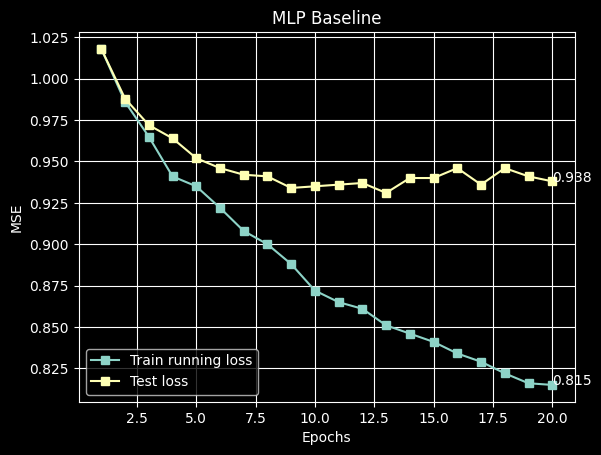
\includegraphics[width=0.6\textwidth]{images/mlp.png}
    \label{fig:mlp}
\end{figure}

\paragraph{LSTM} Our LSTM with 1 million parameters trained in the same way achieved a very similar test loss of 0.91 before starting to overfit.
The  mean squared error train and test loss of the LSTM model trough the $50$ epochs can be seen in figure \ref{fig:lstm}.
\begin{figure}[H]
    \caption{}
    \centering
    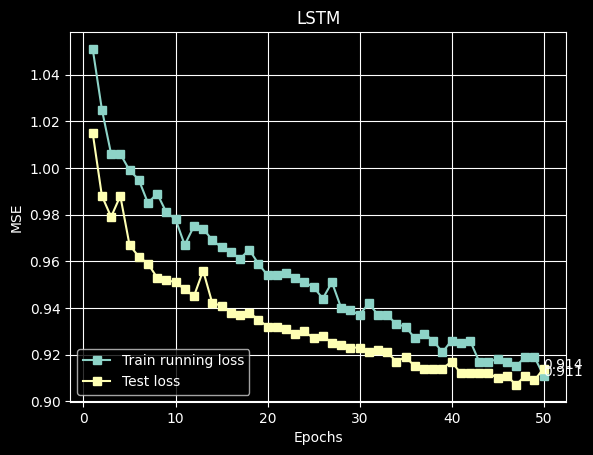
\includegraphics[width=0.6\textwidth]{images/lstm.png}
    \label{fig:lstm}
\end{figure}


Both of these architectures had their hyperparameters tuned extensively to find an acceptable result, but neither of them worked.

\paragraph{Transformer} We then implemented a transformer architecture modified to work on a regression problem. Although this model was bigger at 1.8M parameters, it achieved much better results, ending with a test loss of 0.15, a very promising result. The  mean squared error train and test loss of the Transformer model trough the $40$ epochs can be seen in figure \ref{fig:transformer}.

\begin{figure}[H]
    \caption{}
    \centering
    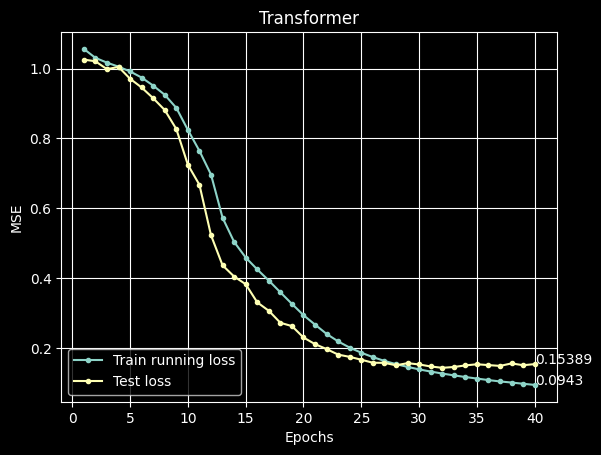
\includegraphics[width=0.6\textwidth]{images/transformer.png}
    \label{fig:transformer}
\end{figure}


All models were trained by intervals of 10 epochs, until they started overfitting. They were not stopped at the same time. 

\paragraph{Scaling} Given the small size of our model, the small size of our dataset and the know scaling properties of transformer models, the promising result of our transformer indicates that we may achieve near-perfect prediction of free energy with a larger set of training examples and a larger model.

\paragraph{Larger Model} To test this hypothesis, we trained a larger transformer model with 8M parameters (about 4 times bigger), on the same dataset. It achieved a test MSE of 0.12, a slightly better result. This represents a 20\% reduction of the Mean Squared Error compared to the smaller model. However, this model's hyperparameters were not optimized due to lack of time. We were also unable to test our transformer model on a larger dataset due to lack of time.


\section{Analysis}
\subsection{Comparison of our models}
In Figure \ref{fig:comparaison}, you can see each of the test loss of the tree models on the same graphic. Both the MLP and LSTM models performed poorly, with the LSTM generalising a bit better. However, there is a key difference between the evolution of the train and test loss for both of these models which can be observed in their respective figures \ref{fig:mlp} and \ref{fig:lstm}. The poor score of the MLP does not seem to be mostly explained by its lack of expressivity, since it manages to get an MSE loss of $0.815$ on the train data, while the LSTM only manages to get an MSE loss of $0.911$. We can hypothesise that the fact that the LSTM still manages to generalise better than the MLP on unseen data implies better bias of the LSTM for our task distribution than the MLP, but a lacking expressivity. \\

\begin{figure}[H]
    \caption{}
    \centering
    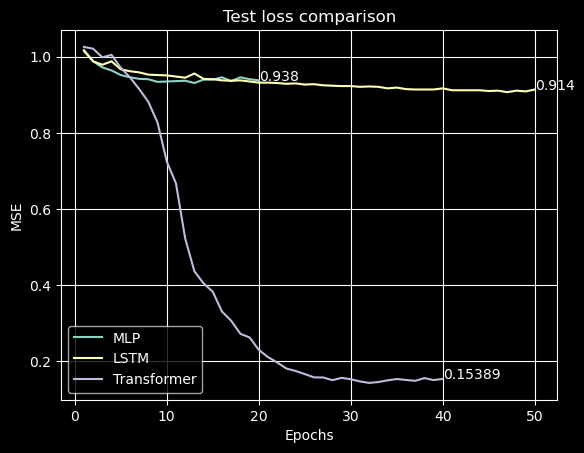
\includegraphics[width=0.6\textwidth]{images/comparaison.png}
    \label{fig:comparaison}
\end{figure}

In contrast, the performance of the Transformer indicates that it has both a good bias towards our task distribution and a sufficient capacity. When introducing the Transformer and the LSTM, we explained several of their respective key features. Though large parts of these networks are black boxes past training, we can still intuit some of the bias they might have towards different tasks when analysing their respective architectures. This is why they were discussed in the methodology in moderate detail. The fact the the Transformer performed so much better indicates that Gibbs Free Energy has less to do with a sequential, stack based distribution. Indeed, the results indicate that in order to predict it, it is more useful to pay attention to several key structural dependencies in the strand, which the Transformer provides explicitely in its architecture, and therefore is most biased towards. In order to better the scores, some regularisation techniques such as orthogonality constraints \cite{zhang-etal-2021-orthogonality} could be added in the cost function of the Transformer. This technique encourages bigger differences in the attention heads during the training by adding a stricly increasing cost term with respect to the orthogonality of the different matrices sued to generate the linear token transformations.


In order to make more conclusive statements about the superiority of Transformers for our task, we would of had to make more costly experiments by training an LSTM with more expressivity. 



\subsection{Transformer Performance on Different Quarters of Our Dataset}
To better understand the strengths and weaknesses of our large transformer model, a more thorough analysis of its predictions follows:

Note: Because the model overfitted before the weights were saved, the MSE for this analysis is 0.15, as opposed to the better result of 0.12 that was mentioned earlier.

On average, our model underestimates the free energy of a strand by 0.27 and the variance of its predictions is 24\% higher than that of the true values. For further analysis, our results were split into four quarters, going from the lowest free energy label to the highest one. The lowest quarter had the worst performance, with a MSE of 0.35. The second lowest was similar to the overall result, with a loss of 0.15. The second highest had a much better result, with a MSE of 0.08, and the highest one was even better at 0.03. These numbers show that our model performs much better on strands with high free energy.

Figure \ref{fig:distri_values} presents the distribution of the free energy labels in our dataset and an analysis of its variance shows that it is skewed towards high free energy values, thus the variance in high free energy strands is much lower than in low free energy strands. This means that for each high energy strand, the model has trained on many more strands with a similar free energy than it has for a lower energy strand. This suggests that increasing the number of training examples would greatly increase the performance of our model, in particular if they are filtered to make a more uniform distribution of free energy labels in the training dataset.

\begin{figure}[H]
    \caption{}
    \centering
    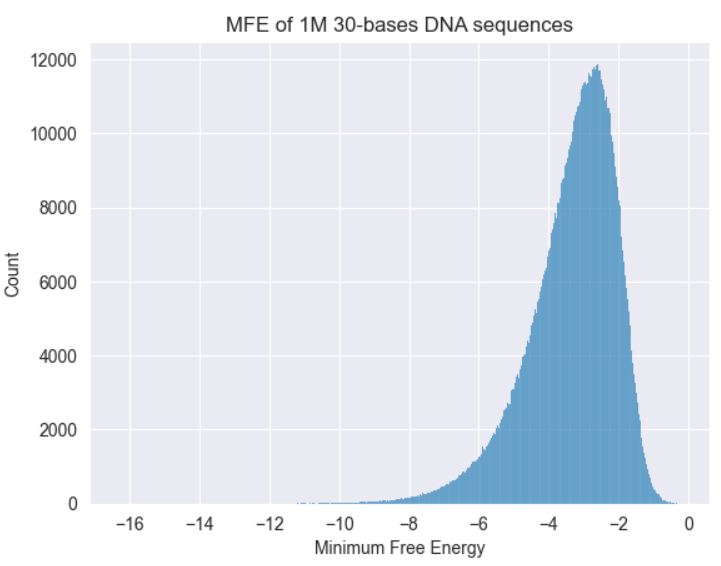
\includegraphics[width=0.5\textwidth]{images/MFE_nupack.png}
    \label{fig:distri_values}
\end{figure}

\section{Conclusion}
Lets briefly summarize our project. First, we were given a regression task involving Aptamers, which are a subset of DNA strands. Using Python, we generated 1 million random DNA strands of length $30$. Then, we used NUPACK's classical algorithm (accessible through a Python API) in order to get predictions of the Gibbs Free Energy of each of these strands. Thus, we had formed our dataset. We then split this dataset into a training set (which contains $90\%$ of the initial dataset) and validation set (which contains $10\%$ of the initial dataset). We then trained several deep neural networks to replicate the classical algorithm from NUPACK, including a Multi Layer Perceptron (our baseline model), a Long Short Term Memory reccurent network and a Transformer. The LSTM network produced slightly better predictions than the MLP baseline model, while the Transformer network performed significantly better than the other two. In our analysis, we briefly provided hypothesis as to the reasons of the aforementionned fact, and provided future suggestions to get obtain a better model based on an examination of our training data. Correctly predicting the stability of higher-dimensional structures from single-stranded aptamers has the potential to not only revolutionize the aptamer-engineering process but also to bolster the range of application for aptasensors in more difficult environments \cite{jeddi2017three}. We believe that our attempt to implement more advanced deep learning architectures such as RNNs and transformers has not only been successful, but also has "potentially" boldly pushed the boundaries of the aptamer-engineering field of research. We expect further curvatures in the loss function to emerge as our best model's is scaled in size and kindly invite our colleagues to validate this hypothesis\footnote{Please do not consider this statement with the utmost seriousness.}.

\section{Contributions of Each Member}
It is difficult to draw straight lines in the stand indicating each contribution of the separate members. Since we set up a well organised GitHub repository, each composite of the project was built like an iterative stack of contributions by each member. Still, we tried to roughly estimate the contributions of each member for each task in Table \ref{tab:contrib}.

\begin{table}[H]
    \centering
    \caption{}
    \begin{tabular}{|c|c|c|c|}
    \hline \\
    Tasks & Guillermo & Jonas & Dereck \\
    \hline \\
     Project coordination & 30 \% & 30\% & 40\% \\
     Constructive critism & 70 \% & 15 \% & 15 \% \\
     Research on Aptamers & 60\% & 25\% & 15\% \\
     Generation of the dataset & 10\% & 80\% & 10\% \\
     MLP Baseline & 0\% & 100\% & 0\% \\
     LSTM & 30 \% & 70 \% & 0\% \\
     Transformer & 0 \% & 20 \% & 80\% \\
     Results & 30\% & 35\% & 35\% \\
     Analysis & 0 \% & 50\% & 50\% \\
     \hline
    \end{tabular}
     \label{tab:contrib} 
\end{table}
\section{Source Code}

The source code for this project can be found at this \href{https://github.com/ScierKnave/dna_aptamers_modelling}{github repository}.
\bibliography{bibliography}
\bibliographystyle{plain}
\end{document}